\subsubsection{Erstes Laden}
\label{Erstes Laden}
Das Sequenzdiagramm zeigt den Ablauf des ersten Ladens beim Aufruf der Webanwendung. Vordergründig soll dabei dargestellt werden, wie die einzelnen Klasseninstanzen erstellt werden. Da es sich um einen Erstbesuch handelt, wird eine Instanz der Klasse CookieNotice erstellt und geöffnet. Das Erstellen der Map Overlays, das in der Methode addOverlay() des Sequenzdiagramms aufgerufen wird, ist im folgenden Sequenzdiagramm dargestellt. 
\begin{center}
	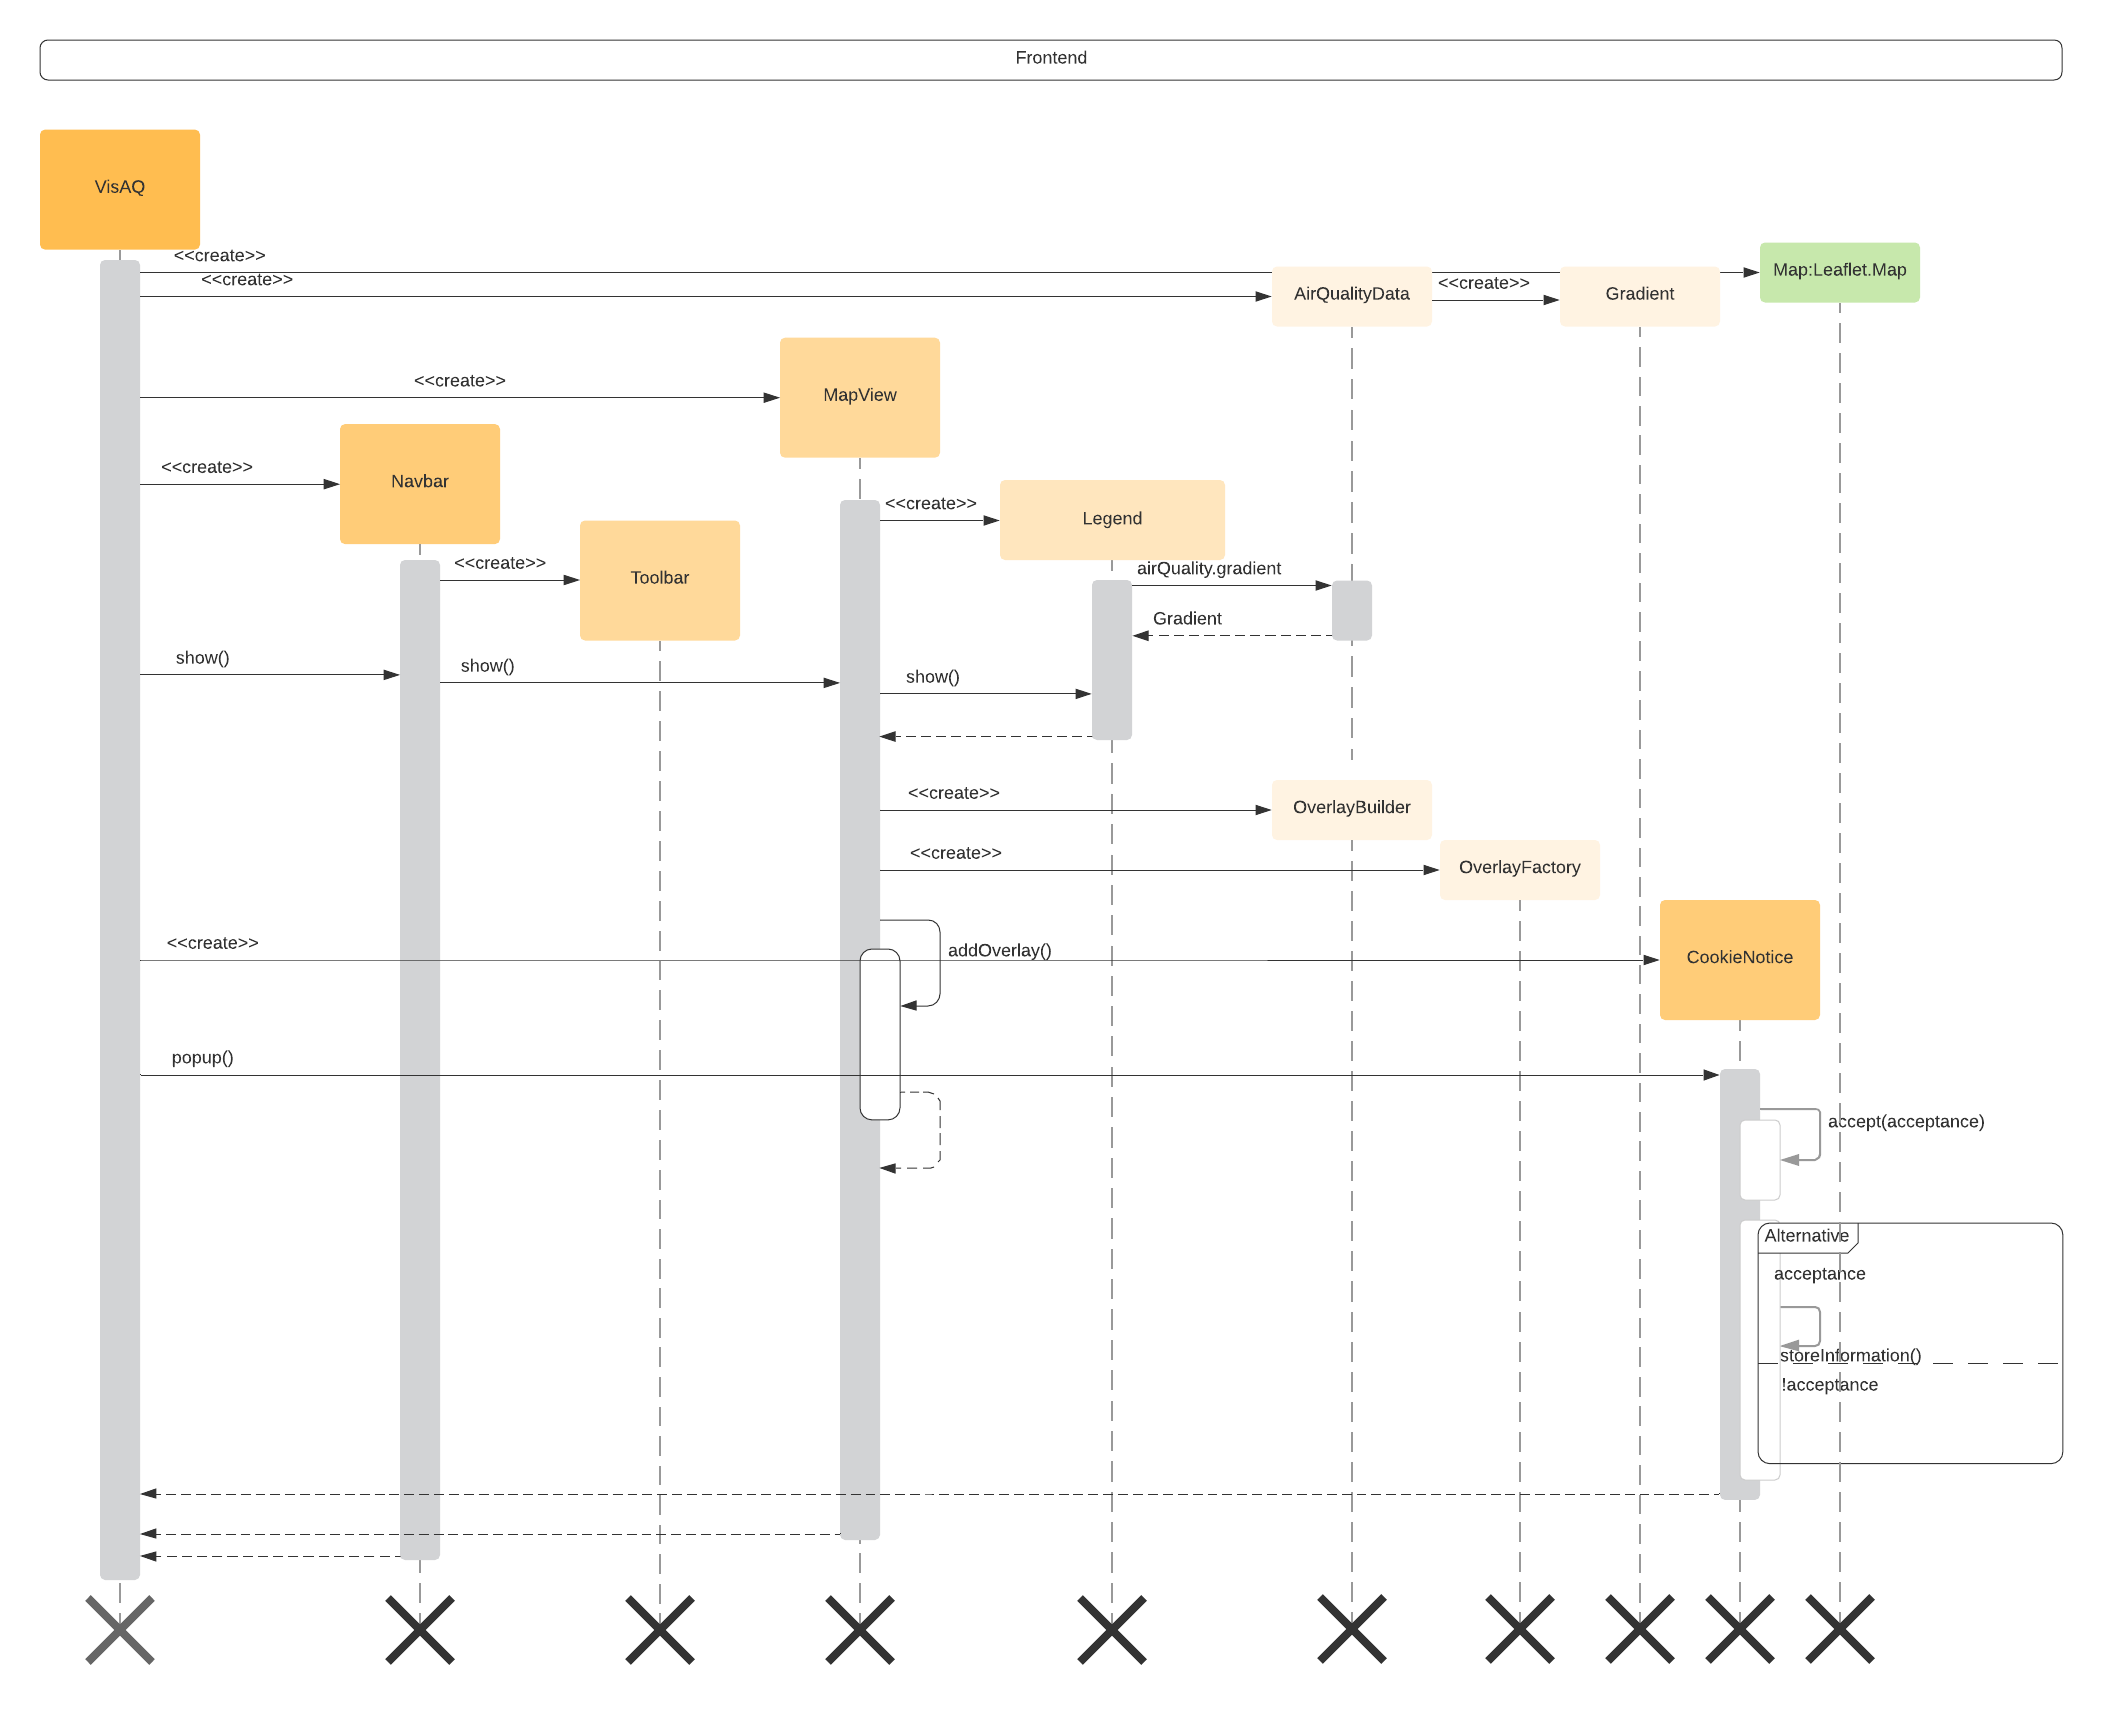
\includegraphics[width=1.2\textwidth]{media/frontend/sequence-diagram/sequenceFirstLoad.png}\captionof{figure}{Erstes Laden} 
\end{center}
\clearpage %opt
\subsubsection{Overlay Factory}
\label{Screenshots}
Das Sequenzdiagramm zeigt den Ablauf zum Erstellen neuer Map Overlays. Ausgelöst wird der Prozess duch das Aufrufen der addOverlay() in MapView. Auf dem OverlayBuilder, der mit den Factories für die gewünschten Map Overlays (z.b Sensor Overlay) instanziiert wurde, wird build() mit den entsprechenden Parametern aufgerufen. Der OverlayBuilder stellt über den AngularController eine Anfrage ans Backend. Mit den erhaltenen Daten beauftragt der OverlayBuilder die Overlay Factories. Die so erstellten Map Overlays gibt der OverlayBuilder an den MapView zurück. Dort werden veraltete Map Overlays von der Map entfernt und die neuen Map Overlays zu Map hinzugefügt. 
\begin{center}
	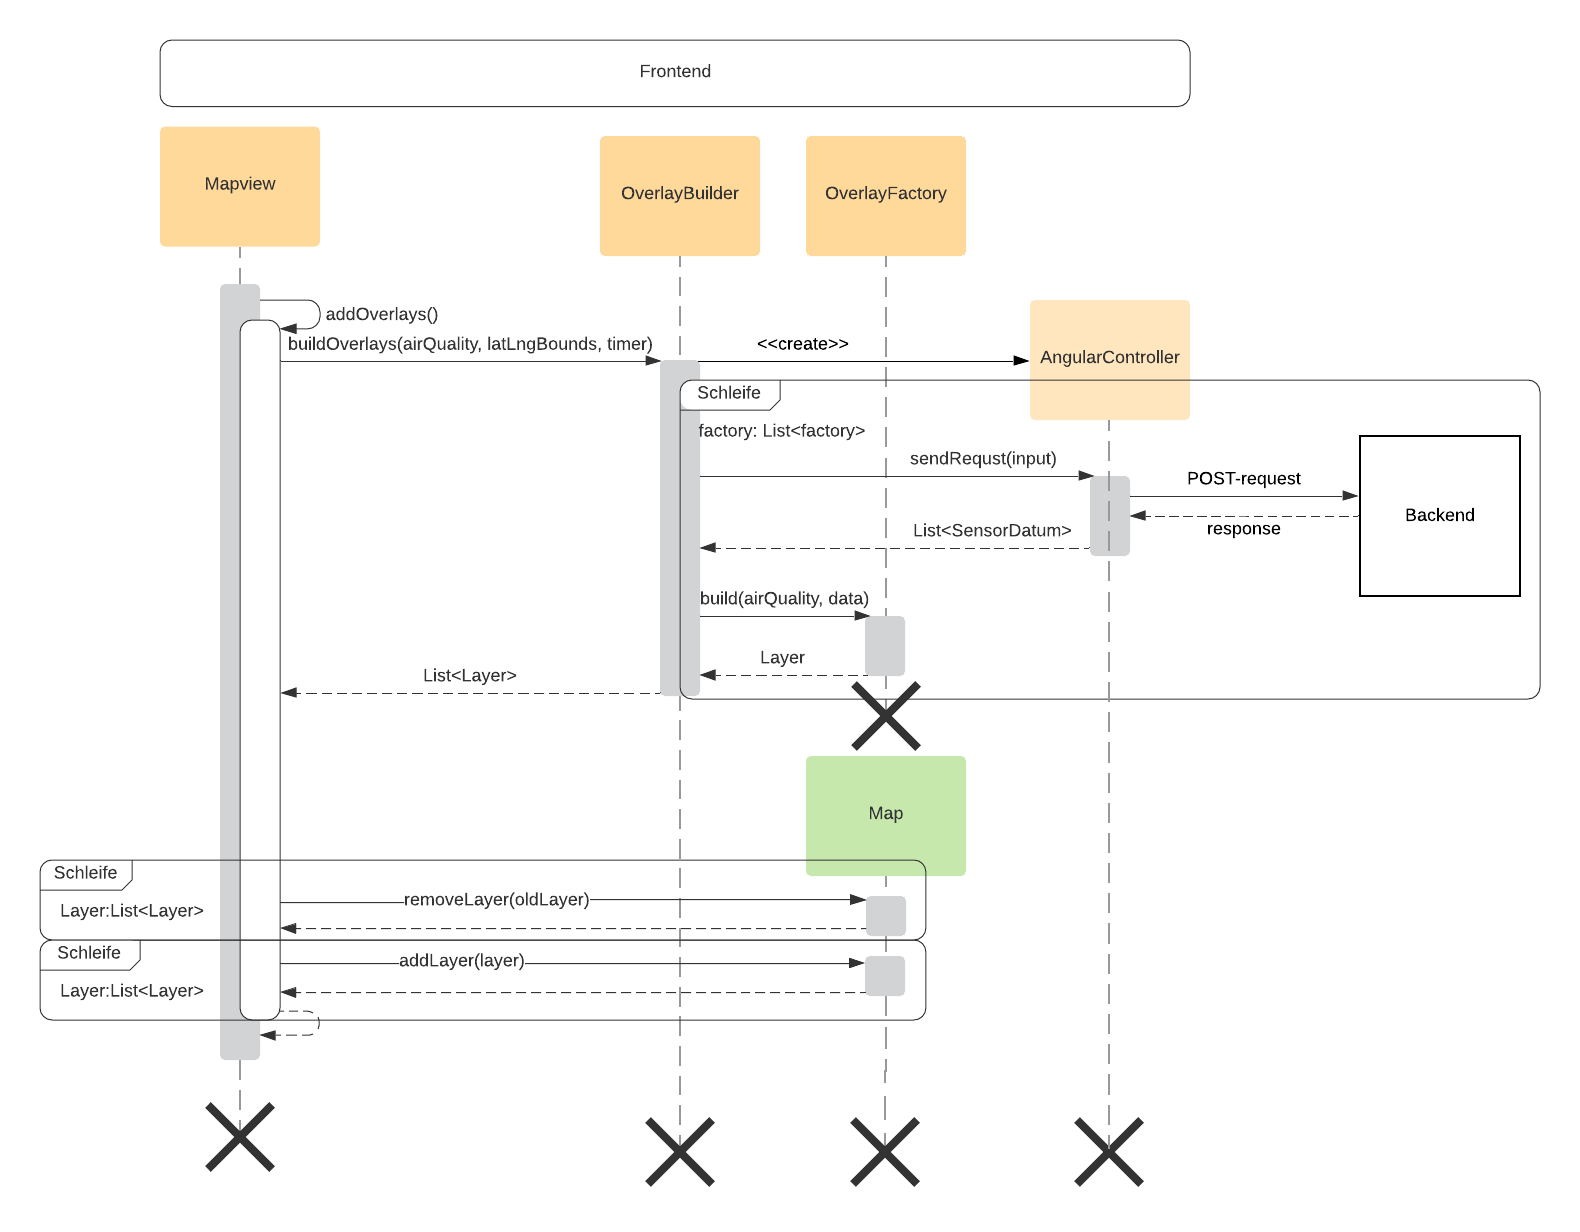
\includegraphics[width=1\textwidth]{media/frontend/sequence-diagram/sequenceOverlayFactory.png}\captionof{figure}{Overlay Factory} 
\end{center}

\subsubsection{Sensor Overview}
\label{Screenshots}
 Das Sequenzdiagramm zeigt den Ablauf beim Laden der Sensor Overview. Aktiviert wird dieser Vorgang durch den Nutzer, der einen Sensor oder einen Punkt auf der Karte markiert. In der MapView wird daraufhin eine neue SensorOverView ertstellt. Die SensorOverview stellt eine Anfrage an das Backend zu den erhaltenen Koordinaten. Mit den Daten aus dem Backend wird ein Diagramm erstellt und auf der SensorOverview dargestellt.
\begin{center}
	\includegraphics[width=1\textwidth]{media/frontend/sequence-diagram/sequenceSensorOverView.png}\captionof{figure}{SensorOverview} 
\end{center}
\clearpage %opt
\subsubsection{SearchBar}
\label{Screenshots}
Das Sequenzdiagramm zeigt den Ablauf beim Suchen eines Ortes über die SearchBar. Der Nutzer gibt hierzu einen existierenden Ort in die SerachBar ein. Die SearchBar informiert die Klasse VisAQ, dass es eine Nutzereingabe stattgefunden hat. VisAQ löst dann aus, dass die Navbar sich aktualisiert, alle Daten an die Views weiterleitet und MapView neu lädt. Der weitere Vorgang findet dann in der Klasse MapView statt.
\begin{center}
	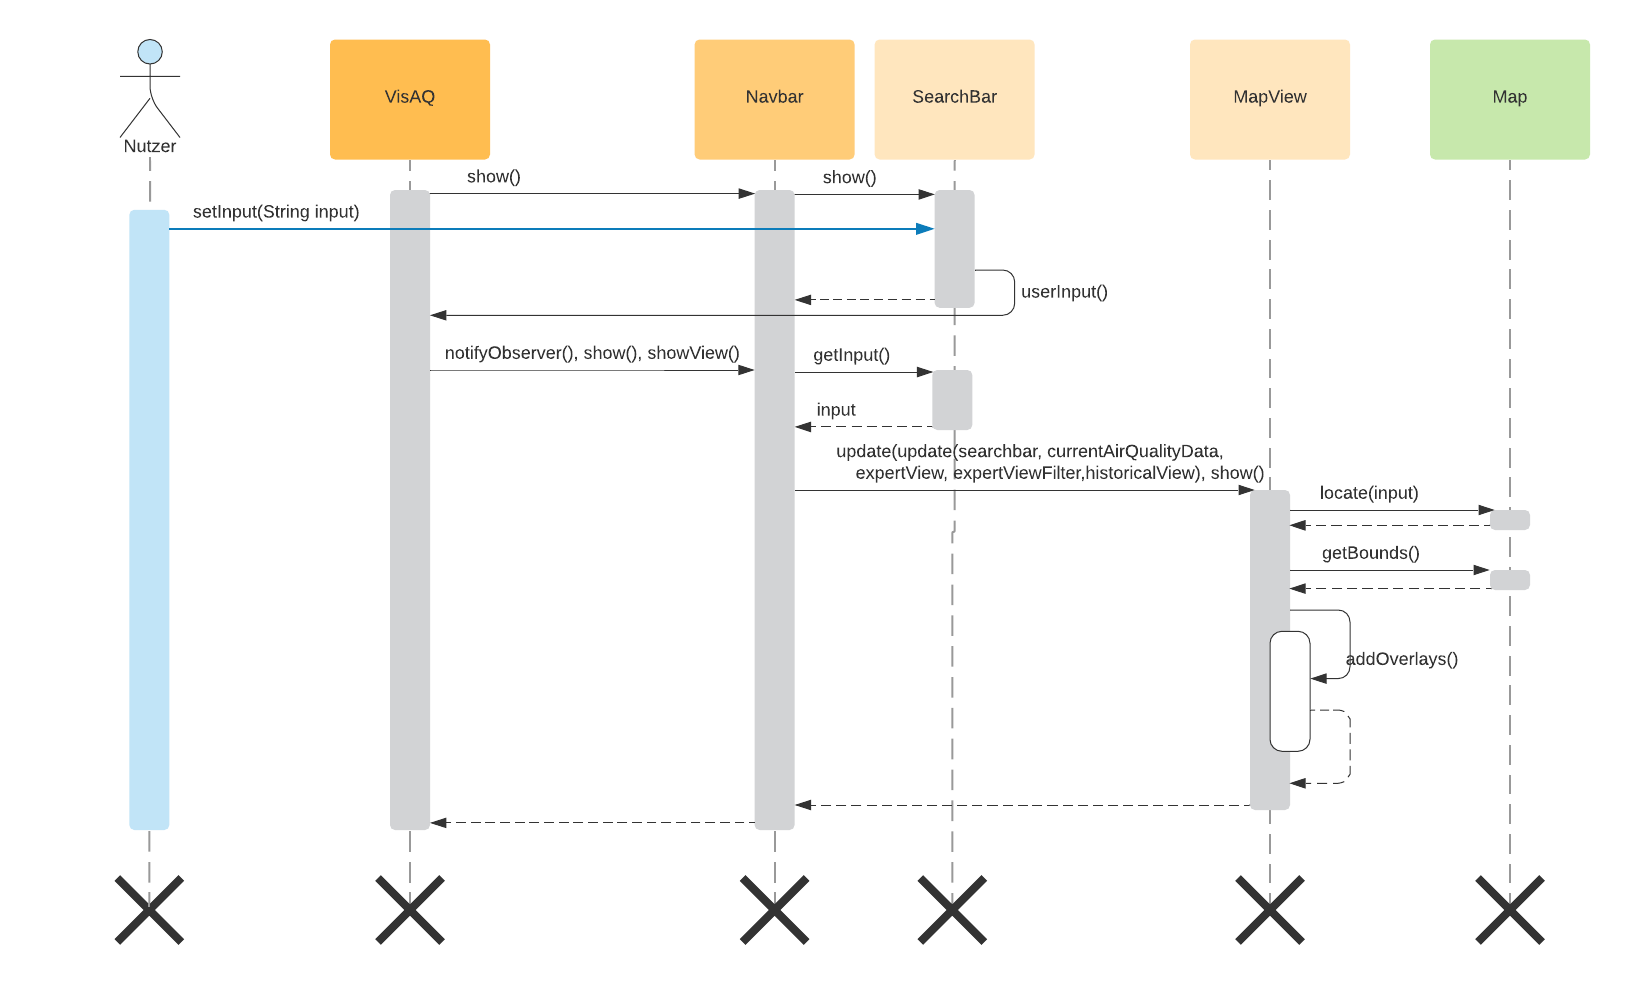
\includegraphics[width=1\textwidth]{media/frontend/sequence-diagram/sequenceSearchbar.png}\captionof{figure}{SearchBar} 
\end{center}
\clearpage %opt
\subsubsection{ColorTheme}
\label{Screenshots}
Das Sequenzdiagramm zeigt den Ablauf, der auf eine Nutzereingabe zur Änderung des Farbschematas folgt.
\begin{center}
	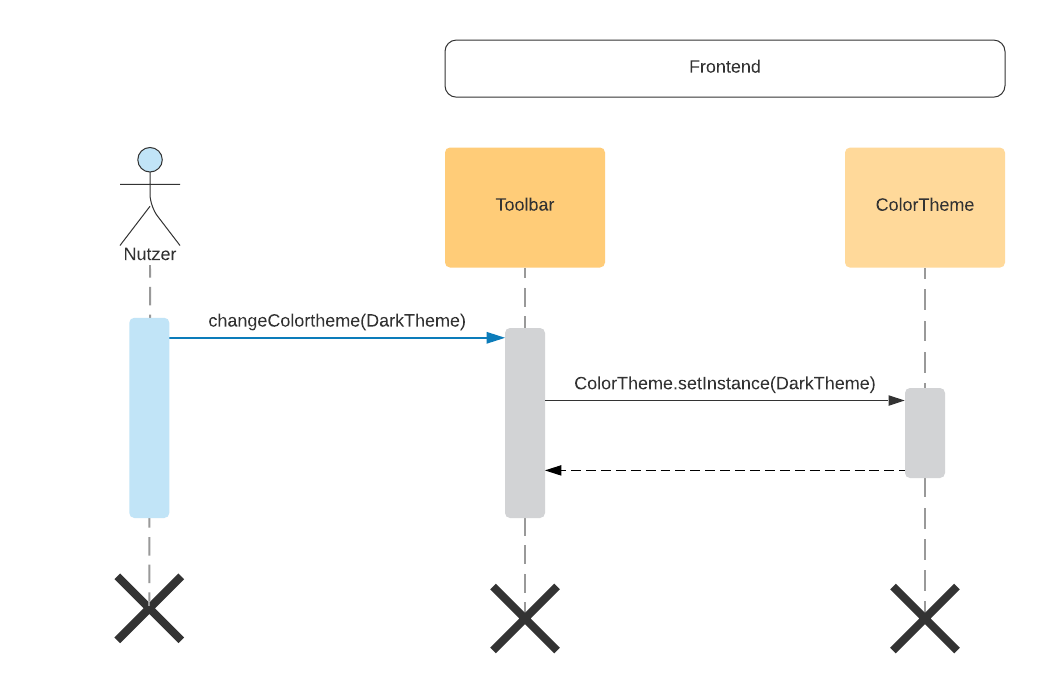
\includegraphics[width=0.8\textwidth]{media/frontend/sequence-diagram/sequenceColorTheme.png}\captionof{figure}{ColorTheme} 
\end{center}
\clearpage %opt
\subsubsection{Multilingual}
\label{Screenshots}
Das Sequenzdiagramm zeigt den Ablauf, der auf eine Nutzereingabe zur Spracheinstellung folgt.
\begin{center}
	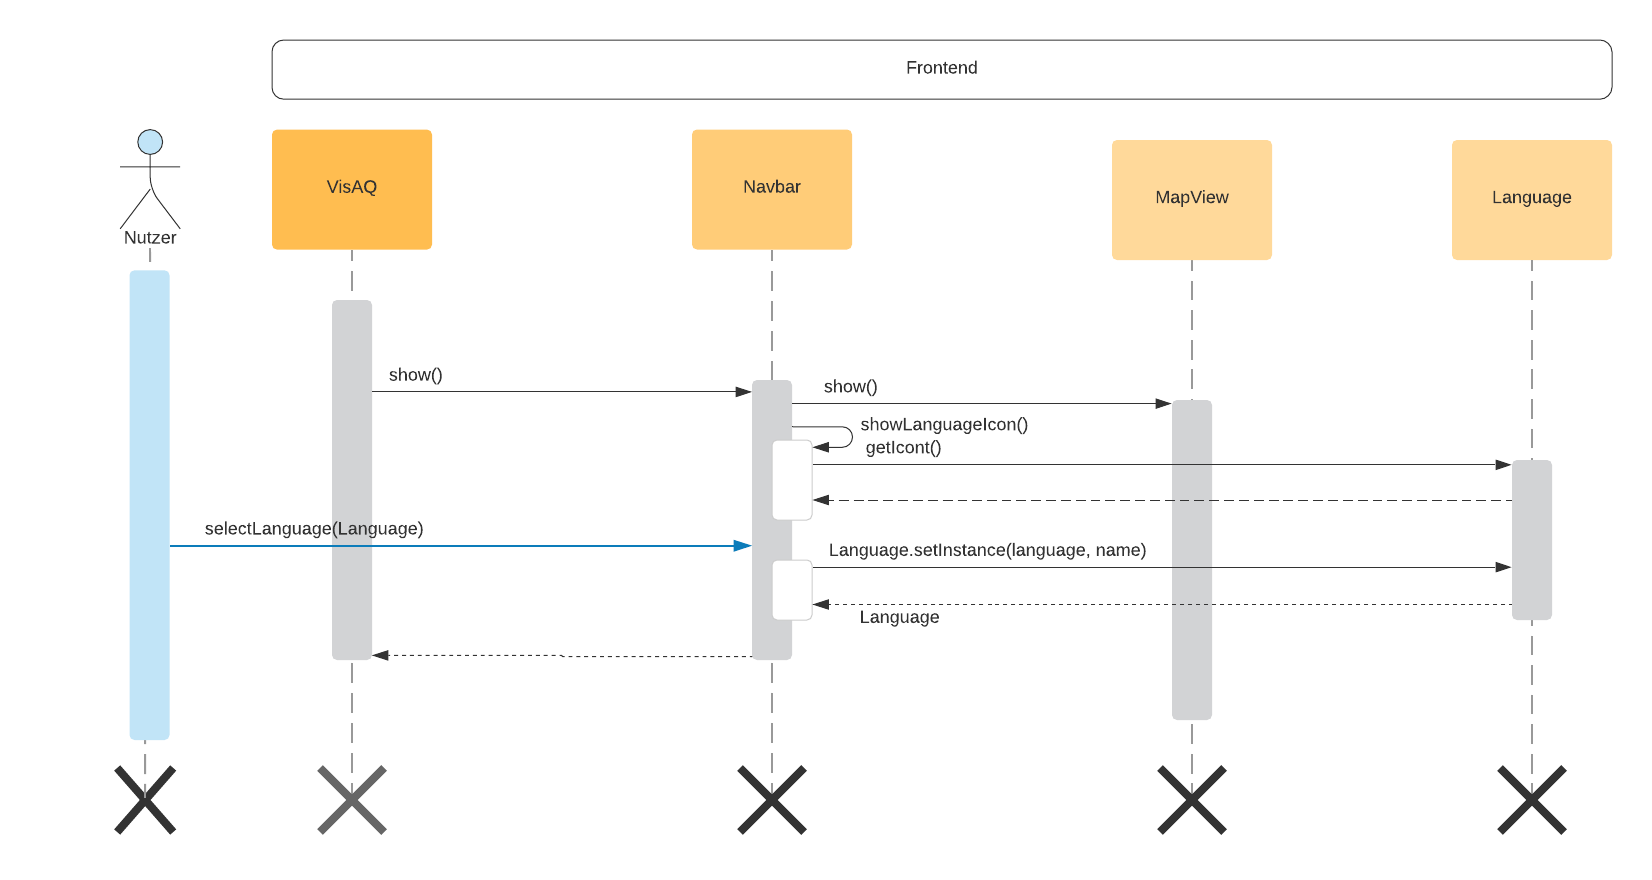
\includegraphics[width=0.9\textwidth]{media/frontend/sequence-diagram/sequenceMultilingual.png}\captionof{figure}{Historical MapView} 
\end{center}

\clearpage %opt
\subsubsection{Expert View}
\label{Screenshots}
Das Sequenzdiagramm zeigt den Ablauf beim Aktivieren des Expert Views. Zunächst wird ein ExpertViewFilter angezeigt, aus welchem der Nutzer die Sensoren auswählen kann, die er sich auf der Karte anzeigen lassen möchte. Mit den ausgewählten Sensoren wird daraufhin eine neue MapView geladen. Hierbei werden dem OverlayBuilder ebenfalls die ausgewählten Sensoren übergeben.
\begin{center}
	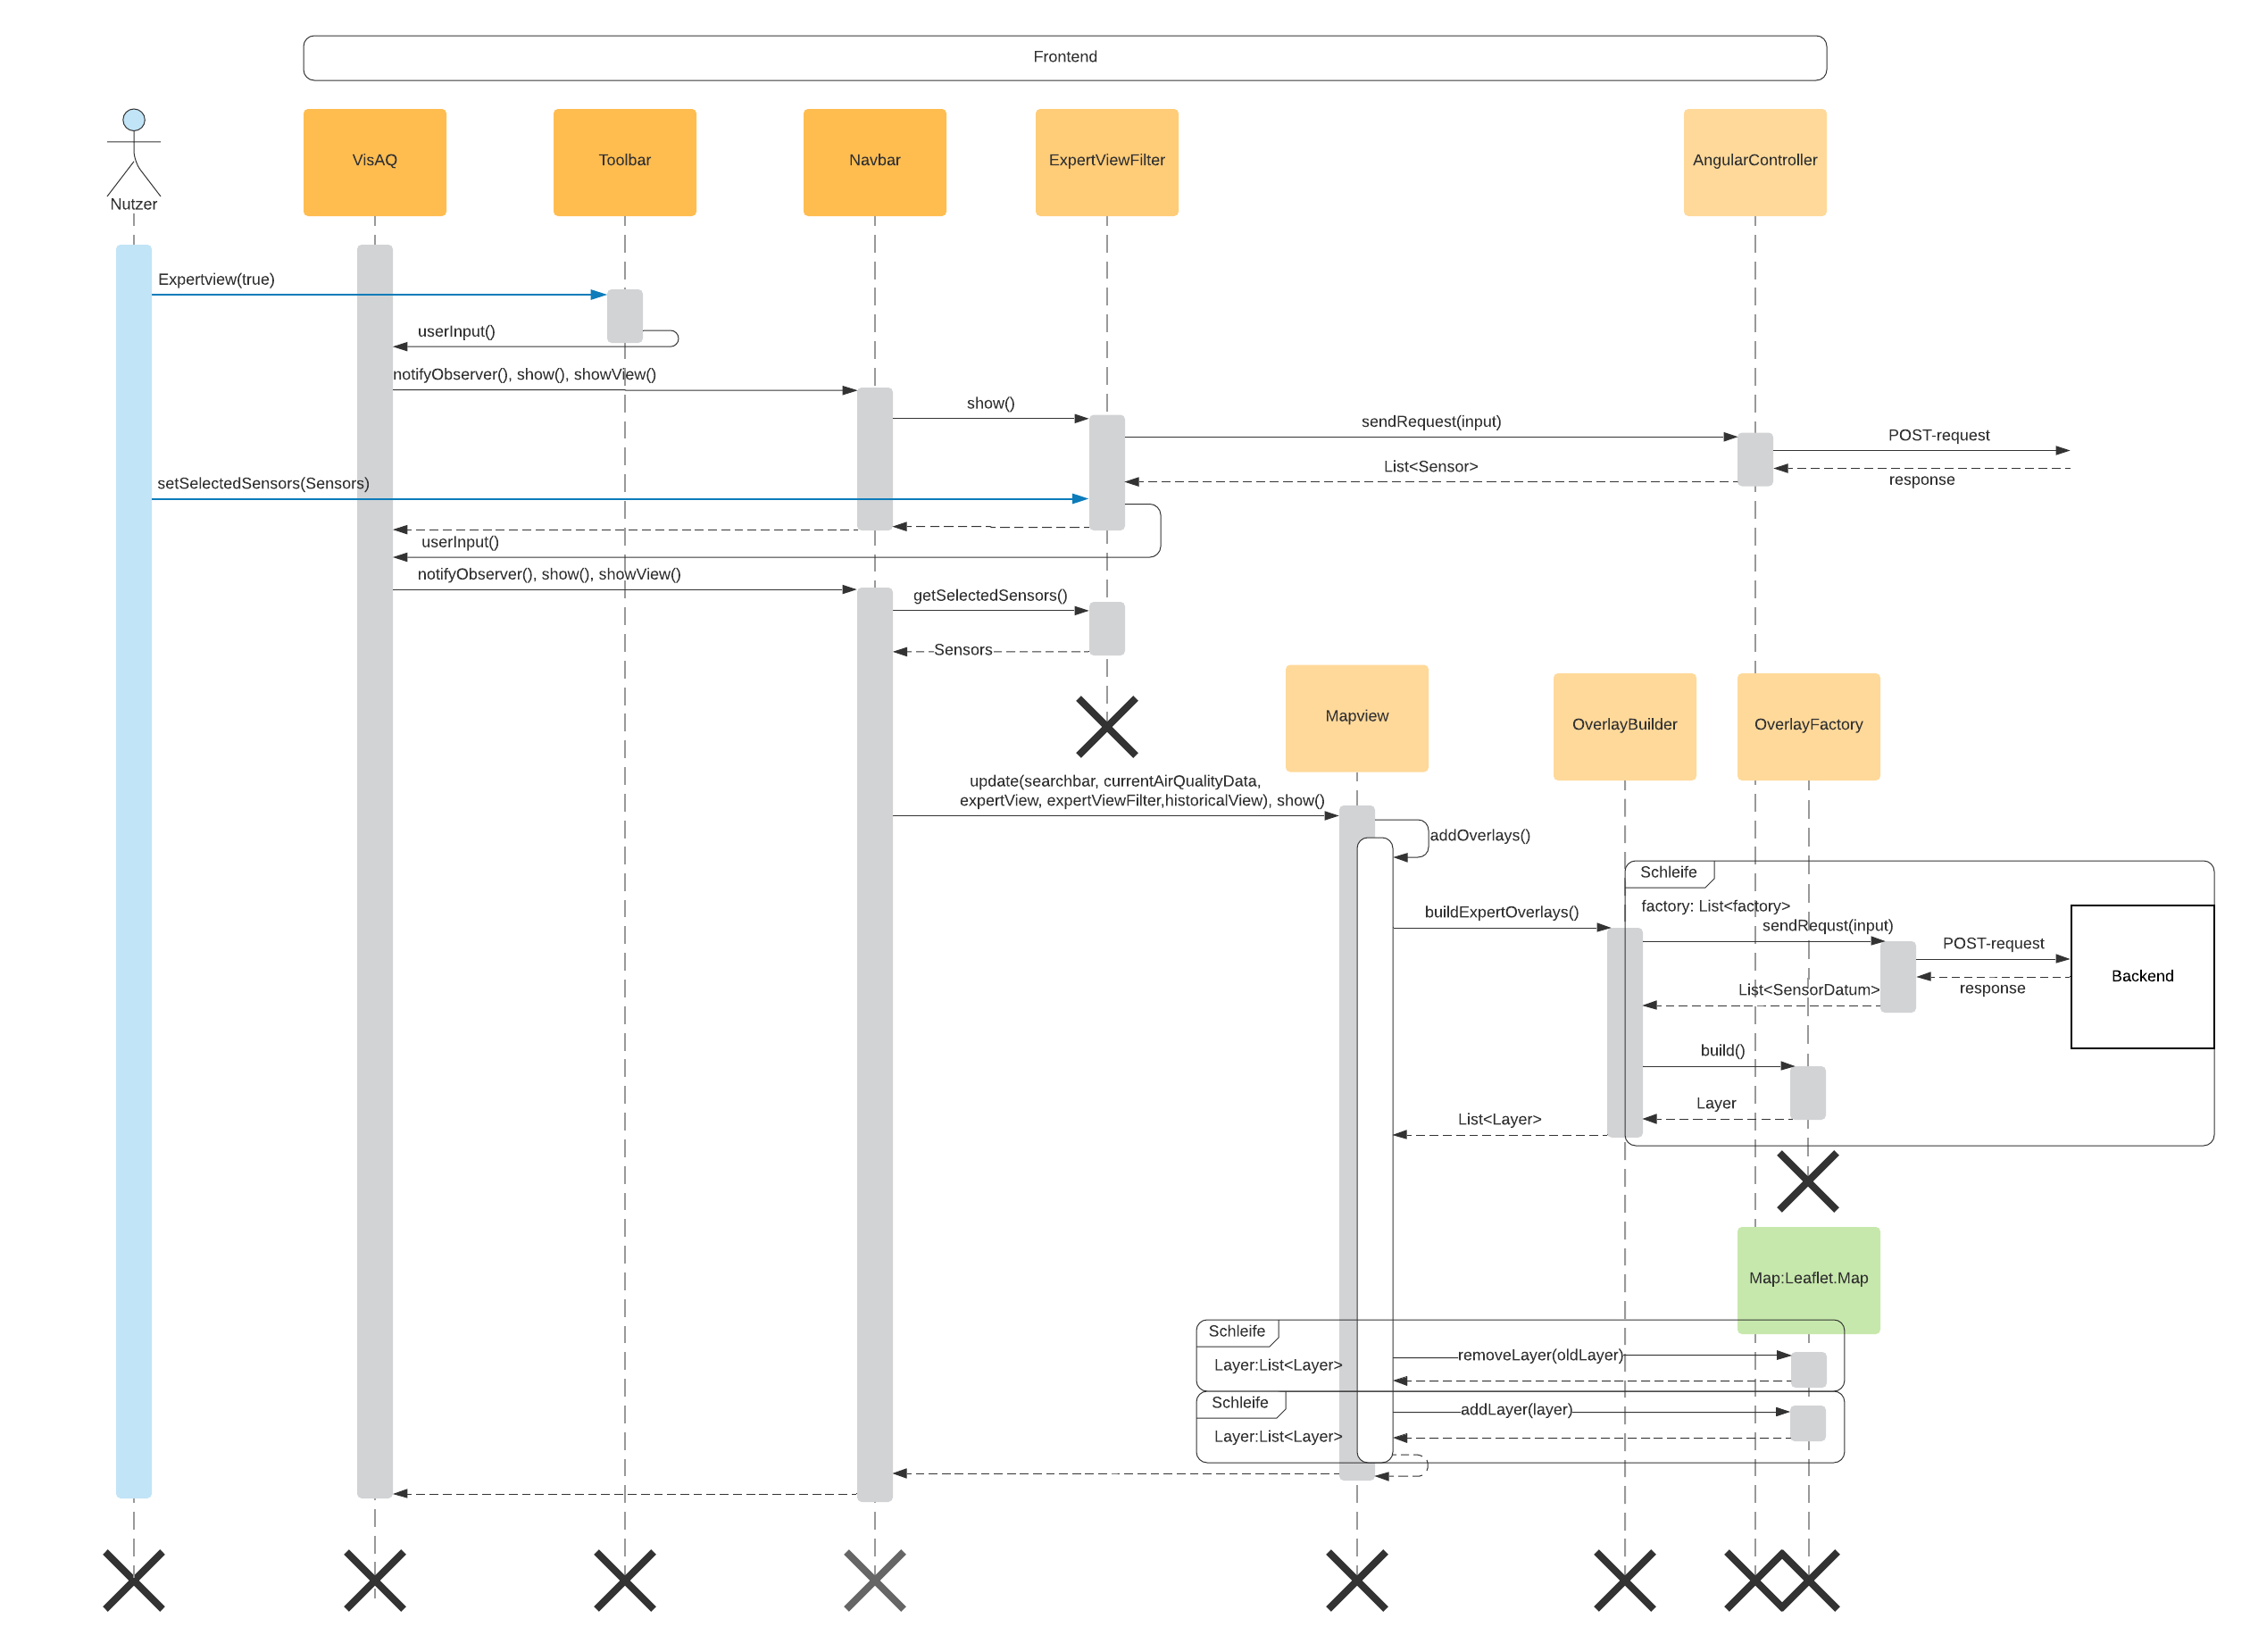
\includegraphics[width=1\textwidth]{media/frontend/sequence-diagram/sequenceExpertViewFilter.png}\captionof{figure}{ExpertView} 
\end{center}


